\section{DQN Traffic Signal Control with Partial Detection}

In this second part, we present the work done during the second half of the internship, which consists of an application project of the DQN algorithm to traffic engineering. Here, we apply DQN to traffic light policy optimization based on limited detected information provided by connected vehicles, which represent a fraction of the total vehicle flow. The contribution is a DQN model for intelligent traffic signal control with partial detection.
The first section formalizes the problem and lays the background, with a review of terminology, literature of related work, and an industry-standard traffic simulation tool. The second section presents the proposed DQN model; DQN-ITSCwPD (DQN Intelligent Traffic Signal Control with Partial Detection), and exposes implementation details of the environment and comparison techniques. The third section presents the training and testing methods, and assesses the model by evaluating the performances over multiple scenarios. Efficiency thresholds are estimated by acceptable and optimal detection rates. \\
The project is available at: \textbf{\url{https://github.com/romainducrocq/DQN-ITSCwPD}}.

\subsection{Background}

In this first section of the second part, we introduce the problem and lay the background foundations, with a literature review of RL and DQN applications to intelligent traffic signal control and partially detected transportation systems. The problem and terminology are first formulated, followed by a review of the current related work and existing tools.

\subsubsection{Problem definition and terminology}

\textbf{Formulation of the problem} \\
We formulate the problem studied in this part and answered with this project as follows: 

\begin{table}[htbp]
\centering
\setlength\tabcolsep{2pt}
\begin{tabular}{|c|}
\hline
\\
\:\:A DQN agent controls the traffic light signals at an isolated intersection\:\:\\
\:\:with the aim to minimize the total travel time through the intersection,\:\:\\
\:\:in a partially observable environment with limited detected information\:\:\\
\:\:provided by a fraction of the total vehicle flow from connected vehicles.\:\:\\
\\
\hline
\end{tabular}
\end{table}

\textbf{Terminology} \\
We define here the transportation theory terminology used throughout this presentation. \\

(1) Network topology and movements:
\begin{itemize}
\setlength\itemsep{-0.5em}
  \item \textbf{Approach}: An approach is a roadway meeting at an intersection, and can be either incoming or outgoing. Vehicles enter the intersection through an incoming approach and leave the intersection through an outgoing approach. For intersections equipped with traffic signal devices, each incoming approach is controlled by a traffic light.
  \item \textbf{Lane}: An approach consists of a set of lanes, which are also either incoming lanes or outgoing lanes. Each incoming lane is controlled by one or many traffic signals.
  \item \textbf{Movement}: A movement refers to a vehicle crossing the intersection from an incoming approach to an outgoing approach, and it is right turn, left turn or through.
  \item \textbf{Connection}: A connection is a link between an incoming lane in an incoming approach and an outgoing lane in an outgoing approach. It enables for a vehicle to perform a movement across the intersection. An incoming lane has a set of connections to one or many outgoing lanes, each controlled by one own traffic signal.
\end{itemize}

(2) Traffic signals and traffic phases:
\begin{itemize}
\setlength\itemsep{-0.5em}
  \item \textbf{Traffic signal}: A traffic signal is a green, yellow or red indication that controls the movements at a connection. Connections are open at green signals, conditionally open at yellow signals and fully closed at red signals, with all movements prohibited.
  \item \textbf{State}: A state is the combination of traffic signals at the intersection, the traffic signals for all the connections of all the incoming lanes of all the incoming approaches.
  \item \textbf{Phase}: A phase is the complete sequence of the successive states and associated time intervals for opening a set of concurrent connections with non-conflicting movements. Phases are intended to separate conflicting connections, so that movements in a phase have no, or minimum, conflicts. A phase consists of a main green interval, either permissive or protected, followed by a change interval and a clearance interval.
  \item \textbf{Green interval}: A green interval, with duration $T_g$, is the first interval in a phase. It allows for some vehicles to cross the intersection along authorized movements from a set of non-conflicting open connections with green traffic signals, while the other connections are closed with red traffic signals. A green interval is either permissive, and conflicting left turns are authorized and made through gaps in oncoming traffic, or protected, and conflicting left turns are not authorized. The green interval is often set to be longer than a minimum green interval, to satisfy driver expectancy, queue clearance, and enable pedestrian crossing in parallel directions, i.e. $T_g \ge T_{g,min}$. 
  \item \textbf{Change interval}: A change interval, with duration $T_y$, follows the green interval as the second interval in a phase. It is a transition interval between two phases of non-conflicting authorized movements, with yellow traffic signals at the set of open connections from the previous green interval,  where vehicles can only cross if they can not stop safely before the stop line, and red traffic signals at other connections.
  \item \textbf{Clearance interval}: A clearance interval, with duration $T_r \ge 0$, is an optional last interval in the phase, and is used to clear the intersection before the green interval of the next phase. All traffic signals are red, and thus all connections are fully closed.
  \item \textbf{Phase interval}: The phase interval is the duration of the phase $T_p = T_g + T_y + T_r$.
  \item \textbf{Cycle}: A cycle is one complete rotation through all the phases at the intersection.
\end{itemize}

(3) Connected vehicles (CV):
\begin{itemize}
\setlength\itemsep{-0.5em}
  \item \textbf{Connected vehicles}: Connected vehicles (CV) are equipped with communication devices and can transmit information to traffic infrastructures, i.e. such as traffic signal controllers, which consists at least of the position and the speed of the vehicle.
  \item \textbf{CV penetration rate}: The connected vehicle penetration rate $p_{cv}$ is the proportion of connected vehicles in the total traffic flow. A mixed traffic comprises of a percentage $p_{cv}$ of connected vehicles and a percentage $1-p_{cv}$ of conventional vehicles.
  \item \textbf{Assumption on CV}: We make the assumption that connected vehicles are fully visible, i.e. their positions and speeds can be observed with perfect accuracy, and conventional vehicles are fully invisible. However, this assumption is debatable; e.g. [11] (Nguyen Van Phu, Farhi, 2020) reports that current GPS localization systems are not precise enough to know the lane in which a CV is situated, but only the approach. They thus provide a probabilistic approach to estimate the lengths of queues in 2-lanes incoming approaches in a mixed traffic scenario. Here, we assume that positions and speeds of CVs are perfectly observable, either through the use of improved technologies or by similar estimation methods applied upstream to data.
\end{itemize}

\subsubsection{Literature review of related work}

\textbf{RL in traffic control} \\
Traffic engineering raises numerous optimal control problems, and as such has been widely studied from the perspective of reinforcement learning. With the main actors of traffic being vehicles, and with the emergence of mixed-autonomy traffic in a near future due to the arrival of automated vehicles, which evolve in road network environments with continuous action spaces, a large portion of the recent studies are addressed by actor-critics and policy-based deep RL algorithms; such as A3C, DDPG, TRPO and PPO.
E.g.; car following on closed networks and shock wave dissipation, lane changing and insertion models, bottleneck decongestion, highway on-ramp merging, and emergent behaviors in mixed-autonomy traffic [12,13,14,15]. Moreover, other traffic actors, such as infrastructures among which traffic lights, present control problems to be optimized in discrete action spaces. This has led researchers to apply DQN algorithms to traffic signal control. \\

\textbf{DQN for traffic signal control} \\
Traffic congestion poses serious economical and social problems; long travelling times, fuel consumption and air pollution; and inefficient traffic signals are significant underlying root causes to the issue. Fixed time traffic signals with predetermined timing have been commonly used, but become inadequate when facing dynamic and varying traffic demands. Thus, with ever growing urban areas and vehicle fleets, adaptive traffic signal control, able to respond to traffic flows in real time, is sought as a major stake of urbanization.
Traffic signal control (TSC) has been addressed by RL methods even before the deep learning era, with Markov chains, dynamic programming, fuzzy logic and discrete tabular Q-learning [16]. However, the advent of deep Q-learning in recent years has enabled to explore many novel TSC applications based on DQN algorithms. Initial studies with simpler models have proven DQN to be efficient for traffic signal control, comparing trained MLP models at isolated intersection with other algorithms from the literature [17,18]. Following studies have build on these models to explore the benefits of complex neural networks architectures, with stacked auto encoders, convolutional neural networks and recurrent neural networks [19,20,21,22,23,24]. Latest work also successfully demonstrated a complete state-of-the-art rainbow DQN implementation for TSC, with adaptations of the six DQN extensions [25]. Furthermore, a significant portion of the research in the field is dedicated to achieve decentralized coordination between traffic lights, with applications of multi agent reinforcement learning (MARL) over up to 1000 coordinated agents [26,27,28,29]. Yet, the main focus and effort in the literature is put on defining state representations and reward functions. Indeed, the complexity of traffic environments, composed of many individual actors interacting together with unpredictable behaviors, leaves these as unresolved questions, with numerous propositions and no overall consensus. \\

\textbf{TSC with connected vehicles} \\
TSC responds to traffic demand based on real time measures of road traffic parameters. While the data are easily recovered in software simulations, real world implementations rely on expensive infrastructures, which exists only at a small fraction of intersections. These are mainly inductive loops under the roads, which allow for macroscopic representations of the traffic, or, in rare cases, radars or video cameras for microscopic descriptions. Most TSC propositions mentioned above require information that are thus difficult to obtain, and are for now mostly inapplicable. However, the rapid  development of IoT has created new technologies applicable for sensing vehicles, such as GPS localization systems, dedicated short ranged communications (DSRC), C-V2X, radio frequency identification, Bluetooth, ultra wide band, Zigbee, and apps (e.g. Google Maps) [11,30]. These communication devices are cost-effective, and do not require heavy infrastructure set ups. An increasing number of equipped connected vehicles are thus nowadays able to transmit their positions and speeds to nearby equipment, allowing for microscopic partial state representations of intersections. Furthermore, latest research have shown that TSC with partial detection applied to CV penetration rates as low as 20\% can significantly improve traffic conditions for all vehicles [31]. These however only consider agents trained over fixed CV penetration rates, which is an unrealistic scenario. DQN applications for TSC with partial detection over connected vehicles have been very little investigated for the time being, and are listed by recent surveys as a gap in the literature and a key future research. \\

\textbf{TSC actions, observations and rewards} \\
The main effort in the literature of TSC with DQN has been placed on the definition of efficient state representations and reward functions. However, RL models are time consuming to tune, and the complexity of TSC environments makes evaluation difficult. Moreover, the issue of reproducibility in RL prevents rigorous comparison of TSC models. Thus, there are for now no widely accepted representations, and many have been proposed. We compile here a non-comprehensive list of agent specifications found in the literature:
\begin{itemize}
\setlength\itemsep{-0.5em}
  \item \textbf{Actions}: Two main types of actions exists; either (1) the TSC agent acyclically selects the next phase from a set of possible phases with fixed green interval duration [17,19,21,24,25,26,27,28,29,30,31,32,33], or (2) the TSC agent selects the duration of the next green interval for the upcoming phase in a predetermined cycle [18,22,23].
  \item \textbf{Observations}: The state representations can either be macroscopic, with estimations of global parameters over traffic flows, or microscopic, with raw data for individual vehicles. While earlier work based on discrete tabular Q-learning or shallow DQN preferred low-dimensional macroscopic state representations, latest work observe individual vehicles for high-dimensional microscopic state representations. Indeed, a significant gain in performance has been measured for microscopic observations over macroscopic ones [32]. Either way, state representations have been usually found to be aggregations of multiple traffic features; among which current phase [18,21,23,26,27,28,29,30,31], number of vehicles [18,23,25,28,30,31,32], positions of vehicles [21,22,23,24,26,32], queue lengths [18,19,23,32,33], speeds of vehicles [17,21,22,32], history of past phases [17,25,32], elapsed time in the current phase [30,31], green, change and clearance intervals duration [30,31], distances to nearest vehicles [30,31], pressures [27,29], number of waiting vehicles [17], waiting times of vehicles [23], and upcoming phase in a cycle [23]; i.e over approaches, lanes or other.
  \item \textbf{Rewards}: The reward functions in TSC, overall, aim at reducing vehicular time loss caused by traffic signals. As such criterion can not be assessed directly, rewards are mostly defined as weighted combinations of traffic features, which coefficients are set empirically. The lack of solid theoretical justifications is a major challenge for real world deployment, as RL rewards are difficult to transcribe mathematically without distorting the intended goal, especially in complex systems. Here, the reward functions act in effect as punishments, and with agents reducing evaluation metrics derived from traffic features, i.e. maximizing negative values; among which delays of vehicles [18,23,26,30,31,32,33], waiting times of vehicles [21,22,23,25,26], queue lengths [19,23,28,33], intersection throughput [17,23,25,33], phase changes [23,25,26], pressures [27,29], accumulated waiting times of vehicles [24], number of waiting vehicles [25], travel times of vehicles [23], emergency stops  of vehicles [26], and teleports of vehicles (in Sumo) [26]; i.e. over approaches, lanes or other, and over cumulative values, averages, relative differences, individual vehicles, or other. 
\end{itemize}

\pagebreak

\newgeometry{left= 3cm, right= 2cm, bottom= 0cm, top= 2.6cm}

\subsubsection{Traffic simulation with Sumo}

\textbf{Traffic simulators as RL environments} \\
Traffic networks are complex stochastic environments, where many actors concurrently evolve in a shared space, i.e. vehicles, pedestrians, infrastructures. At the particle scale, the uncoordinated interactions between drivers with conflicting interests, each minimizes its travel time, create unpredictable behaviors. At the global scale, they are bound by the laws of traffic flow physics and dynamics, with perturbations propagated and amplified. Hence, TSC relies on the use of industry-standard software traffic simulators, based on microscopic mathematical models and differential calculus over longitudinal and lateral vehicle dynamics [12]. These allow to develop RL control strategies with high-fidelity state representations, and test them over large and heterogeneous road networks and scenarios. The main traffic simulators used in the TSC research community are Sumo, Aimsum, Cityflow, Paramics and Matsim [34]. As part of this project, we use the Sumo simulator. \\

\textbf{SUMO, Simulation of Urban MObility} \\
Sumo (simulation of urban mbility) [35], is an open source, microscopic, continuous and industry-standard traffic simulation software and package of tools for modeling large road networks with high fidelity, developed by the German Aerospace Center (DLR) since 2001. \\ 
It allows for complex scenario generation with decentralized and multi modal simulated objects, including vehicles, pedestrians and infrastructures. Traffic scenarios are designed in a set of \texttt{XML} configuration files, where simulation data are specified, i.e. they define (1) network structures with intersections, approaches, lanes and connections, (2) traffic demands with vehicle insertion times and routes, and (3) traffic lights with signal programs; and can be created in the visual network editor \texttt{netedit}. Networks can be both synthetic, or converted from real world OSM data. Furthermore, Sumo comes with two python code interfaces to embed the simulated environment within larger programs, the \texttt{sumolib} and \texttt{traci} libraries. These contain modules and functions for interacting online with simulations in real time, and provide control over the simulated networks and agents. Sumo can be used either from the command line interface with simulations over sub processes, or with a graphical user interface, with the \texttt{sumo} and \texttt{sumo-gui} packages.

\begin{figure}[h]
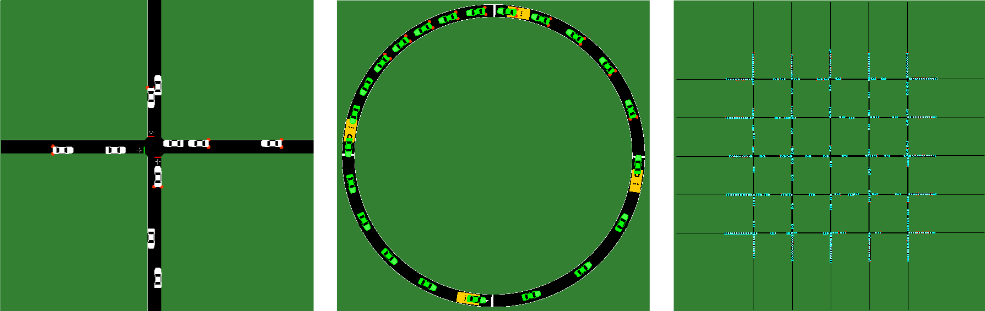
\includegraphics[width=\textwidth]{img/II/Selection_111.png}
\centering
\captionsetup{justification=centering}
\caption{Sumo GUI visuals.}
\end{figure}

\restoregeometry

\pagebreak